\documentclass{article}
\usepackage{amsmath} % Required for typesetting matrices
\usepackage{amssymb} % Required for using the "therefore" symbol
\usepackage{graphicx}

\title{Matrix, Linear Algebra, Differential Equation \\ MAT 2207}
\author{Jannat Tohfa Chowdhury}
\date{April 2024}

\begin{document}
\maketitle
\newpage
% Your lectures start here
\section*{Matrix}
\subsection*{Definition of Matrix: }
\vspace{10pt}
A system of any \( m \times n \) numbers arranged in a rectangular arrangement of \( m \) rows and \( n \) columns is called a matrix of order \( m \times n \) or an \( m \times n \) matrix.
    \paragraph{Ex:}
    \[
    \begin{minipage}{0.6\textwidth}
    \[
    \begin{bmatrix}
    1 & -2 & 4 \\
    3 & 1 & 7 \\
    \end{bmatrix}
    \]
    \end{minipage}
    \begin{minipage}{0.4\textwidth}
    is a $2 \times 3$ matrix.
    \end{minipage}
    \]
    \vspace{12pt}
    \textbf{in general form:}
    \[
    A = 
    \begin{bmatrix}
    \sigma_{11} & \sigma_{12} & \cdots & \sigma_{1n} \\
    \sigma_{21} & \sigma_{22} & \cdots & \sigma_{2n} \\
    \vdots & \vdots & \vdots & \vdots \\
    \sigma_{m1} & \sigma_{m2} & \cdots & \sigma_{mm}
    \end{bmatrix}
    =(\sigma_{ij})_{mxm}
    \]
\vspace{20pt}
\subsection*{Singular and Non-singular Matrix:}
\vspace{10pt}
    Let \( A \) be any square matrix. If \( \det(A) = 0 \), then \( A \) is called a singular matrix, and if \( \det(A) \neq 0 \), then \( A \) is called a non-singular matrix.
    \vspace{12pt}
    \paragraph{Ex:}
    \begin{minipage}{0.4\textwidth}
    \[ A = 
    \begin{bmatrix}
    1 & 2 \\
    2 & 4 \\
    \end{bmatrix} \]
    \end{minipage}
    \begin{minipage}{0.1\textwidth}
    \end{minipage} 
    \begin{minipage}{0.4\textwidth}
    \[ B = 
    \begin{bmatrix}
    1 & 5 \\
    2 & 12 \\
    \end{bmatrix} \]
    \end{minipage}

    \vspace{20pt}    
    Then \(|A| = \det(A) = \det \begin{bmatrix} 1 & 2 \\ 2 & 4 \end{bmatrix} = 4 - 4 = 0\)
    
    So, \(A\) is a singular matrix
    
    \vspace{20pt}
    Again, \(|B| = \det(B) = \det \begin{bmatrix} 1 & 5 \\ 2 & 12 \end{bmatrix} = 12 - 10 = 2 \neq 0\)
    
    Hence, \( B \) is a non-singular matrix.
\vspace{20pt}
\subsection*{Inverse Matrix:}
\vspace{10pt}
    Let \( A \) and \( B \) be two \(n \times n\) square matrices such that \( AB = BA = I_{n} = I \), then \( B \) is said to be the inverse of \( A \), and we write \( B = A^{-1} \). Also, \( A = B^{-1} \).
    \vspace{20pt}
    \paragraph{Ex:}
    Let \( A = \begin{bmatrix} 4 & 3 \\ 1 & 1 \end{bmatrix} \) and \( B = \begin{bmatrix} 1 & -3 \\ -1 & 4 \end{bmatrix} \).
    
    \vspace{10pt}
    
    \begin{minipage}{.45\textwidth}
    \(\therefore\ AB = 
    \begin{bmatrix} 4 & 3 \\ 1 & 1 \end{bmatrix}
    \times
    \begin{bmatrix} 1 & -3 \\ -1 & 4 \end{bmatrix}\)
    \end{minipage}

    
    \vspace{10pt}
    
    \begin{minipage}{0.7\textwidth}
    \[ = \begin{bmatrix} 4 - 3 & -12 + 12 \\ 1 - 1 & -3 + 4 \end{bmatrix} = \begin{bmatrix} 1 & 0 \\ 0 & 1 \end{bmatrix} = I_{2} \]
    \end{minipage}
    
    \vspace{10pt}
    
    \begin{minipage}{0.6\textwidth}
    and \( BA = \begin{bmatrix} 1 & -3 \\ -1 & 4 \end{bmatrix} \times \begin{bmatrix} 4 & 3 \\ 1 & 1 \end{bmatrix} \)
    \end{minipage}
    
    \vspace{10pt}

    \begin{minipage}{0.7\textwidth}
        \[ = \begin{bmatrix} 4 - 3 & 3 - 3 \\ -4 + 4 & -3 + 4 \end{bmatrix} = \begin{bmatrix} 1 & 0 \\ 0 & 1 \end{bmatrix} = I_{2} \]
    \end{minipage}
   
    \vspace{10pt}
    
    \(\therefore\)\(AB = BA = I_{2} = I\)
    
    Therefore, we can write \( A = B^{-1} \) and \( B = A^{-1} \).

    \vspace{30pt}
    [N.B.: The inverse of a matrix exists only when the matrix is non-singular,

i.e., \( |A| \neq \emptyset \).]

    *** Multiplication of two matrices is possible only when the number of columns in the first matrix is equal to the number of rows in the second matrix.

\vspace{20pt}

\subsection*{Echelon Matrix:}
    \vspace{10pt}
    Let \( A = (a_{ij})_{m \times n} \) be any matrix. Then \( A \) is said to be an echelon matrix or is said to be in echelon form if:
    \begin{enumerate}
        \item all the non-zero rows (if any) precede the zero rows,
        \item the number of zero entries preceding the first non-zero entry in each row increases by row.
    \end{enumerate}

    \vspace{10pt}

    \paragraph{Ex:}
    \[\begin{bmatrix} 1 & -1 & 2 \\ 0 & 3 & 2 \\ 0 & 0 & 5 \end{bmatrix} \text{ is an echelon matrix,  but } \begin{bmatrix} 1 & 2 & 3 \\ 0 & -1 & 3 \\ 2 & 5 & 4 \end{bmatrix} \text{ is not an echelon matrix.}\]

    \vspace{20px}

\subsection*{Rank of a Matrix:}
    \vspace{10pt}
    Rank of a matrix is the largest non-zero row in the matrix of row echelon form.

    \paragraph{Ex:}
    \begin{minipage}{0.45\textwidth}
    \[ A = \begin{bmatrix} 1 & 4 & 5 \\ 0 & 3 & 7 \\ 0 & 0 & 6 \end{bmatrix} \]
    \end{minipage}
    \begin{minipage}{0.45\textwidth}
        \[ B = \begin{bmatrix} 1 & 2 & 3 \\ 0 & 6 & 7 \\ 0 & 0 & 0 \end{bmatrix} \]
    \end{minipage}

    \vspace{20pt}
    \text{Rank of matrix } A = 3, \quad \text{Rank of matrix } B = 2

    \vspace{60pt}
    \textbf{Find the rank of the following matrices:}
    
    \begin{center}
    \begin{minipage}{0.45\textwidth}
    \[ A = \begin{bmatrix} 1 & -1 & -1 & 2 \\ 2 & 1 & 3 & -1 \\ 3 & 2 & 1 & 2 \\ 4 & 1 & 2 & 3 \end{bmatrix} \]
    \end{minipage}
    \hspace{0.05\textwidth}
    \begin{minipage}{0.45\textwidth}
    \[ B = \begin{bmatrix} 1 & 3 & 1 & -2 & -3 \\ 1 & 4 & 3 & -1 & -4 \\ 2 & 3 & -4 & -7 & -3 \\ 3 & 8 & 1 & -7 & -8 \end{bmatrix} \]
    \end{minipage}
    \end{center}
    
    \vspace{1em}
    
    \begin{center}
    \begin{minipage}{0.45\textwidth}
    \[ C = \begin{bmatrix} 1 & -1 & 2 & 1 \\ 3 & 0 & 2 & 2 \\ 2 & 1 & -1 & 1 \\ 1 & 0 & 1 & 1 \end{bmatrix} \]
    \end{minipage}
    \hspace{0.05\textwidth}
    \begin{minipage}{0.45\textwidth}
    \[ D = \begin{bmatrix} 1 & -1 & 1 & 3 \\ 2 & -1 & 0 & 2 \\ 1 & 0 & 1 & 1 \\ 4 & 2 & 0 & 1 \end{bmatrix} \]
    \end{minipage}
    \end{center}

    \vspace{120pt}

    \begin{figure}[htbp]
        \centering
        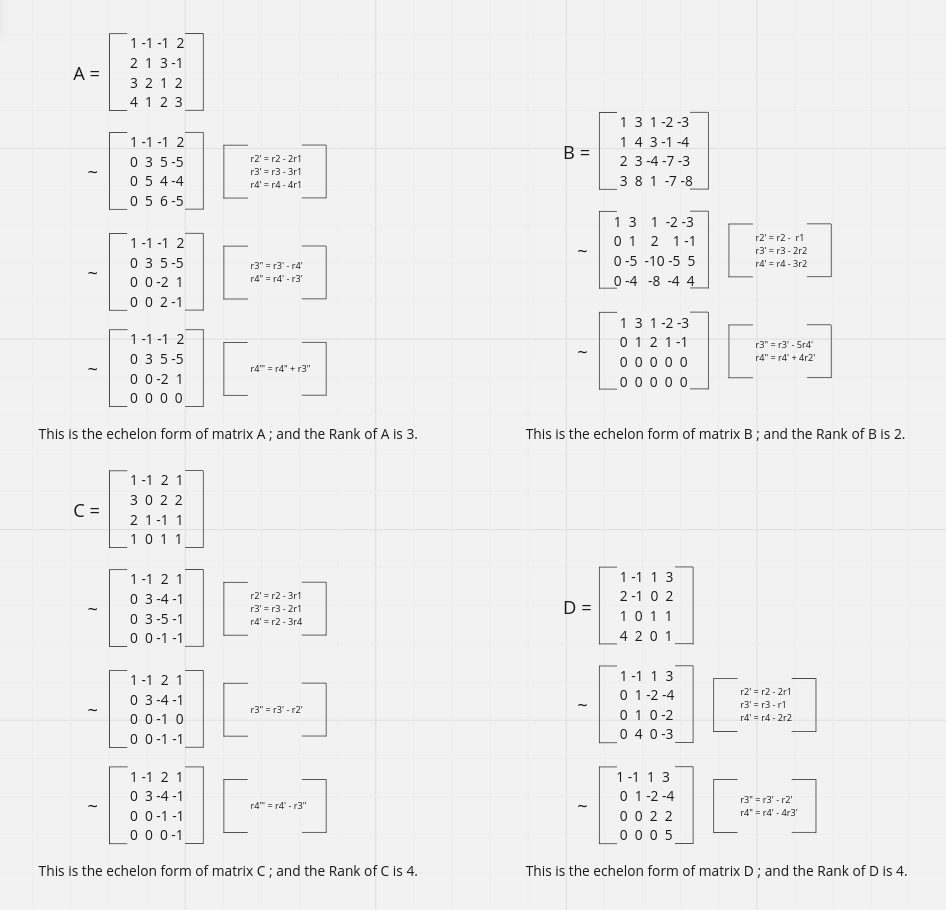
\includegraphics[width=1.2\textwidth, height=.95\textheight]{../Asset/rankOfExc.png}
        \label{fig:example}
    \end{figure}
    
    \newpage
    \section*{Inverse Matrix Calculation:}
    \vspace{10pt}
    Find the inverse of the matrix by using the formula [A:I]

    \vspace{10pt}
    example; find the inverse matrix of \( A = \begin{bmatrix} 1 & -1 & 2 & 1 \\ 3 & 0 & 2 & 2 \\ 2 & 1 & -1 & 1 \\ 1 & 0 & 1 & 1 \end{bmatrix} \)

    \vspace{10pt}
    Solution:
    \vspace{10pt}
    \begin{figure}[htbp]
        \centering
        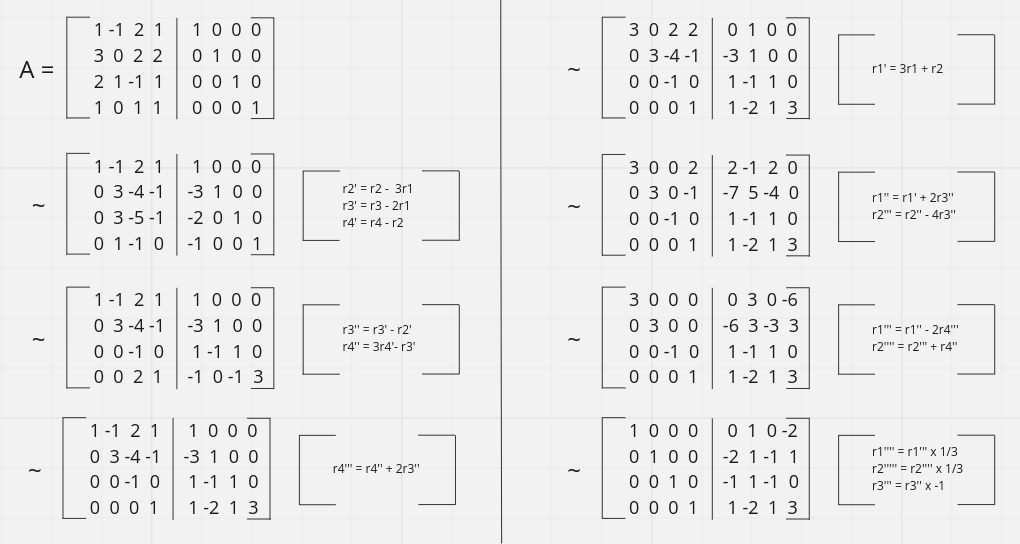
\includegraphics[width=1.2\textwidth, height=.7\textheight]{../Asset/invEXA.png}        \label{fig:example}
    \end{figure}

    \vspace{10pt}
    \newpage
    \underbar{Home Work:}

    find the inverse matrix of
    \hspace*{10pt}
    \( B = \begin{bmatrix} -1 & 2 & -3 \\ 2 & 1 & 0 \\ 4 & -2 & 5 \end{bmatrix} \);  
    \( C = \begin{bmatrix} 1 & 3 & 1 & 1 \\ 2 & 5 & 2 & 2 \\ 1 & 3 & 8 & 9 \\ 1 & 3 & 2 & 2 \end{bmatrix} \)
    
    \begin{figure}[htbp]
        \centering
        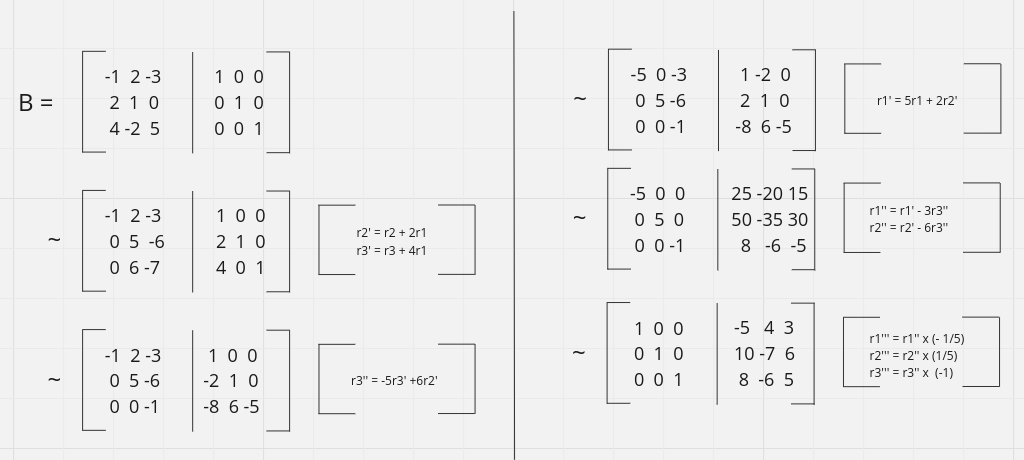
\includegraphics[width=1.2\textwidth, height=.7\textheight]{../Asset/invHWB.png}
        \label{fig:example}
    \end{figure}
    \begin{figure}[htbp]
        \centering
        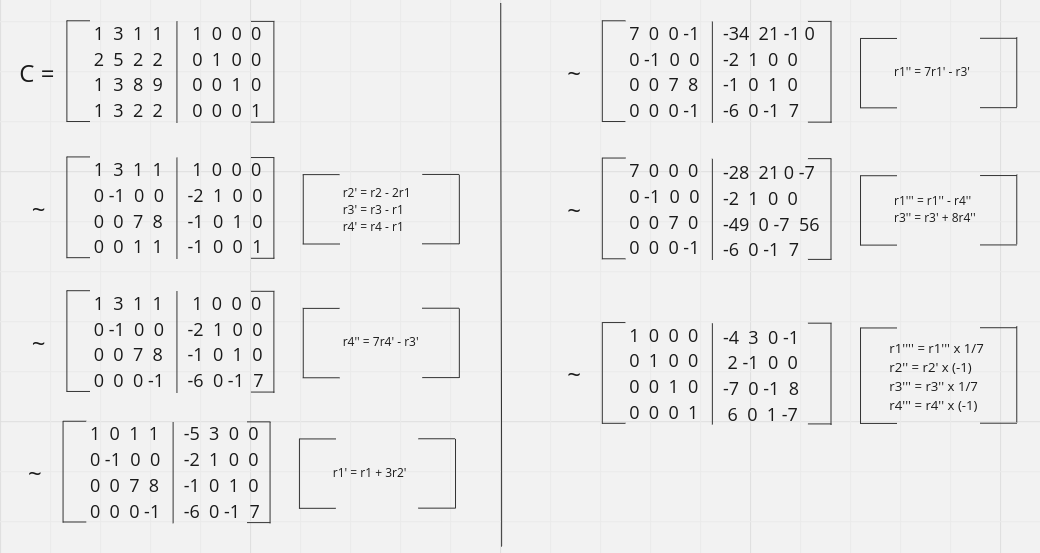
\includegraphics[width=1.2\textwidth, height=.7\textheight]{../Asset/invHWC.png}
        \label{fig:example}
    \end{figure}

    \newpage
    \section*{Eigenvalues and Eigenvectors:}
    
    \vspace{10pt}
    A nonzero matrix \( X \) is an eigenvector of a square matrix \( A \) if there exists a \( \lambda \) such that \( AX = \lambda X \). Then \( X \) is called the eigenvector of \( A \) with eigenvalue \( \lambda \) and \( \lambda \) is called the eigenvalue of \( A \).
    
    \vspace{10pt}
    The equation \( |A - \lambda I| = 0\) is called the characteristic equation of \( A \).
    
    \vspace{10pt}
    Cayley-Hamilton theorem states that every square matrix A satisfies it's characteristic equation.

    \vspace{10pt}
    \subsection*{Example:}
        Find the eigenvalues and eigenvectors of the matrix \( A = \begin{bmatrix} 1 & 4 \\  2 & 3  \end{bmatrix} \) in the field of real numbers ( \( \mathbb{R} \) ). Also verify the Cayley-Hamilton theorem.

    \vspace{20pt}
    \textbf{\underline{\textit{Sol}}$_{\textit{n}}$}:

    \vspace{10pt}
    Given matrix, \(A = \begin{bmatrix} 1 & 4 \\  2 & 3  \end{bmatrix}\)
    
    \vspace{10pt}
    Characteristic matrix of A inverse:

    \[
    \begin{aligned}
        A - \lambda I &= 
        \begin{bmatrix}
            1 & 4 \\
            2 & 3
        \end{bmatrix}
        - \lambda
        \begin{bmatrix}
            1 & 0 \\
            0 & 1
        \end{bmatrix} \\
        &= \begin{bmatrix}
                1-\lambda & 4 \\
                2 & 3-\lambda
            \end{bmatrix}
    \end{aligned}
    \]
    \vspace{20pt}

    Characteristic equation of A inverse:

    \vspace{10pt}
    \(|A - \lambda I| = 0 \)

    or,
    \[
    \left|
    \begin{array}{cc}
        1 - \lambda & 4 \\
        2 & 3 - \lambda
    \end{array}
    \right| = 0
    \]

    or,
    \((1 - \lambda)(3 - \lambda) - 8 = 0 \)

    or,
    \(3 - 4\lambda + \lambda^2 - 8 = 0 \)

    or,
    \( \lambda^2 - 4\lambda - 5 = 0 \)

    or,
    \( \lambda^2 - 5\lambda + \lambda - 5 = 0 \)

    or
    \( \lambda = 1 \) or \( \lambda = -5 \)

    \vspace{10pt}
    thus, \( \lambda = 1, -5 \); 

    these are the eigenvalues of \( A \).

    \newpage

    For \(x = 5\), 

    \[
    \begin{aligned}
        (A - \lambda I) v &= 0 \\
        \text{or,} \quad &\begin{bmatrix}
            1-5 & 4 \\
            2 & 3-5
        \end{bmatrix} \begin{bmatrix}
            x_1 \\
            x_2
        \end{bmatrix} = 0 \\
        \text{or,} \quad &\begin{bmatrix}
            -4 & 4 \\
            2 & -2
        \end{bmatrix} \begin{bmatrix}
            x_1 \\
            x_2
        \end{bmatrix} = 0
    \end{aligned}
    \]
    
    Now, we can write,
    
    \[
    \begin{aligned}
        -4x_1 + 4x_2 &= 0 \\
        2x_1 - 2x_2 &= 0 \\
        \text{or,} \quad &\begin{bmatrix}
            -4 & 4 \\
            2 & -2
        \end{bmatrix} \begin{bmatrix}
            x_1 \\
            x_2
        \end{bmatrix} = \begin{bmatrix}
            0 \\
            0
        \end{bmatrix} \\
        \sim \quad &\begin{bmatrix}
            -4 & 4 \\
            0 & 0
        \end{bmatrix} \quad [r_2' = 2r_2 + r_1] \\
        \sim \quad &\begin{bmatrix}
            -1 & 1 \\
            0 & 0
        \end{bmatrix} \quad [r_1' = r_1 \times \frac{1}{4}]
    \end{aligned}
    \]
    
    \vspace{10pt}
    From this first row,
    
    \[
    \begin{aligned}
        -x_1 + x_2 &= 0 \\
        x_1 &= x_2 = s \quad (\text{say})
    \end{aligned}
    \]
    
    Taking \(s = 1\), the eigenvector can be written as,
    
    \[
    v_1 = \begin{bmatrix}
        1 \\
        1
    \end{bmatrix}
    \]
    
    Now for \(\lambda = -1\),
    
    \[
    \begin{aligned}
        (A - \lambda I) v &= 0 \\
        \text{or,} \quad &\begin{bmatrix}
            1-(-1) & 4 \\
            2 & 3-(-1)
        \end{bmatrix} \begin{bmatrix}
            x_1 \\
            x_2
        \end{bmatrix} = 0 \\
        \text{or,} \quad &\begin{bmatrix}
            2 & 4 \\
            2 & 4
        \end{bmatrix} \begin{bmatrix}
            x_1 \\
            x_2
        \end{bmatrix} = 0
    \end{aligned}
    \]
    
    \newpage
    Now, we can write,
    
    \[
    \begin{aligned}
        &2x_1 + 4x_2 = 0 \\
        &2x_1 + 4x_2 = 0 \\
        \text{or,} \quad &\begin{bmatrix}
            2 & 4 \\
            2 & 4
        \end{bmatrix} \begin{bmatrix}
            x_1 \\
            x_2
        \end{bmatrix} = \begin{bmatrix}
            0 \\
            0
        \end{bmatrix} \\
        \sim \quad &\begin{bmatrix}
            2 & 4 \\
            0 & 0
        \end{bmatrix} \quad [r_2' = r_2 - r_1] \\
        \sim \quad &\begin{bmatrix}
            1 & 2 \\
            0 & 0
        \end{bmatrix} \quad [r_1' = r_1 \times \frac{1}{2}]
    \end{aligned}
    \]
    
    \vspace{10pt}
    From this first row,
    
    \[
    \begin{aligned}
        & x_1 + 2x_2 = 0 \\
        & x_1 = -2x_2
    \end{aligned}
    \]
    
    Taking \(x_2 = 1\), we get \(x_1 = -2\). Thus, the eigenvector can be written as,
    
    \[
    v_2 = \begin{bmatrix}
        -2 \\
        1
    \end{bmatrix}
    \]
    
    \subsection*{Cayley-Hamilton proof: }
    We have to show that \( A^2 - 4A - 5 = 0 \).

    \[
    \left| \text{Det}(A) \right| = \left| \text{Det}\left( \begin{bmatrix} 1 & 4 \\ 2 & 3 \end{bmatrix} \right) \right|
    = |(1 \times 3) - (4 \times 2)| = |3 - 8| = 5
    \]
    
    Thus, 
    \[
    \text{Left side} = A^2 - 4A - 5 = 5^2 - 4 \times 5 - 5 = 25 - 20 - 5 = 0 = \text{Right side} \quad [\text{Proofed}]
    \]
    

\end{document}


